\section{Die DJI Phantom 2 Vision Plus\cite{phantom}}
Die DJI Phantom 2 Vision Plus ist ein Multikopter. Er hat mehrere Rotoren die für den Auftrieb zuständig sind, im Gegensatz zum Helikopter (ein Rotor plus Steuer).
\begin{wrapfigure}{l}{0.6\textwidth}
  \begin{center}
    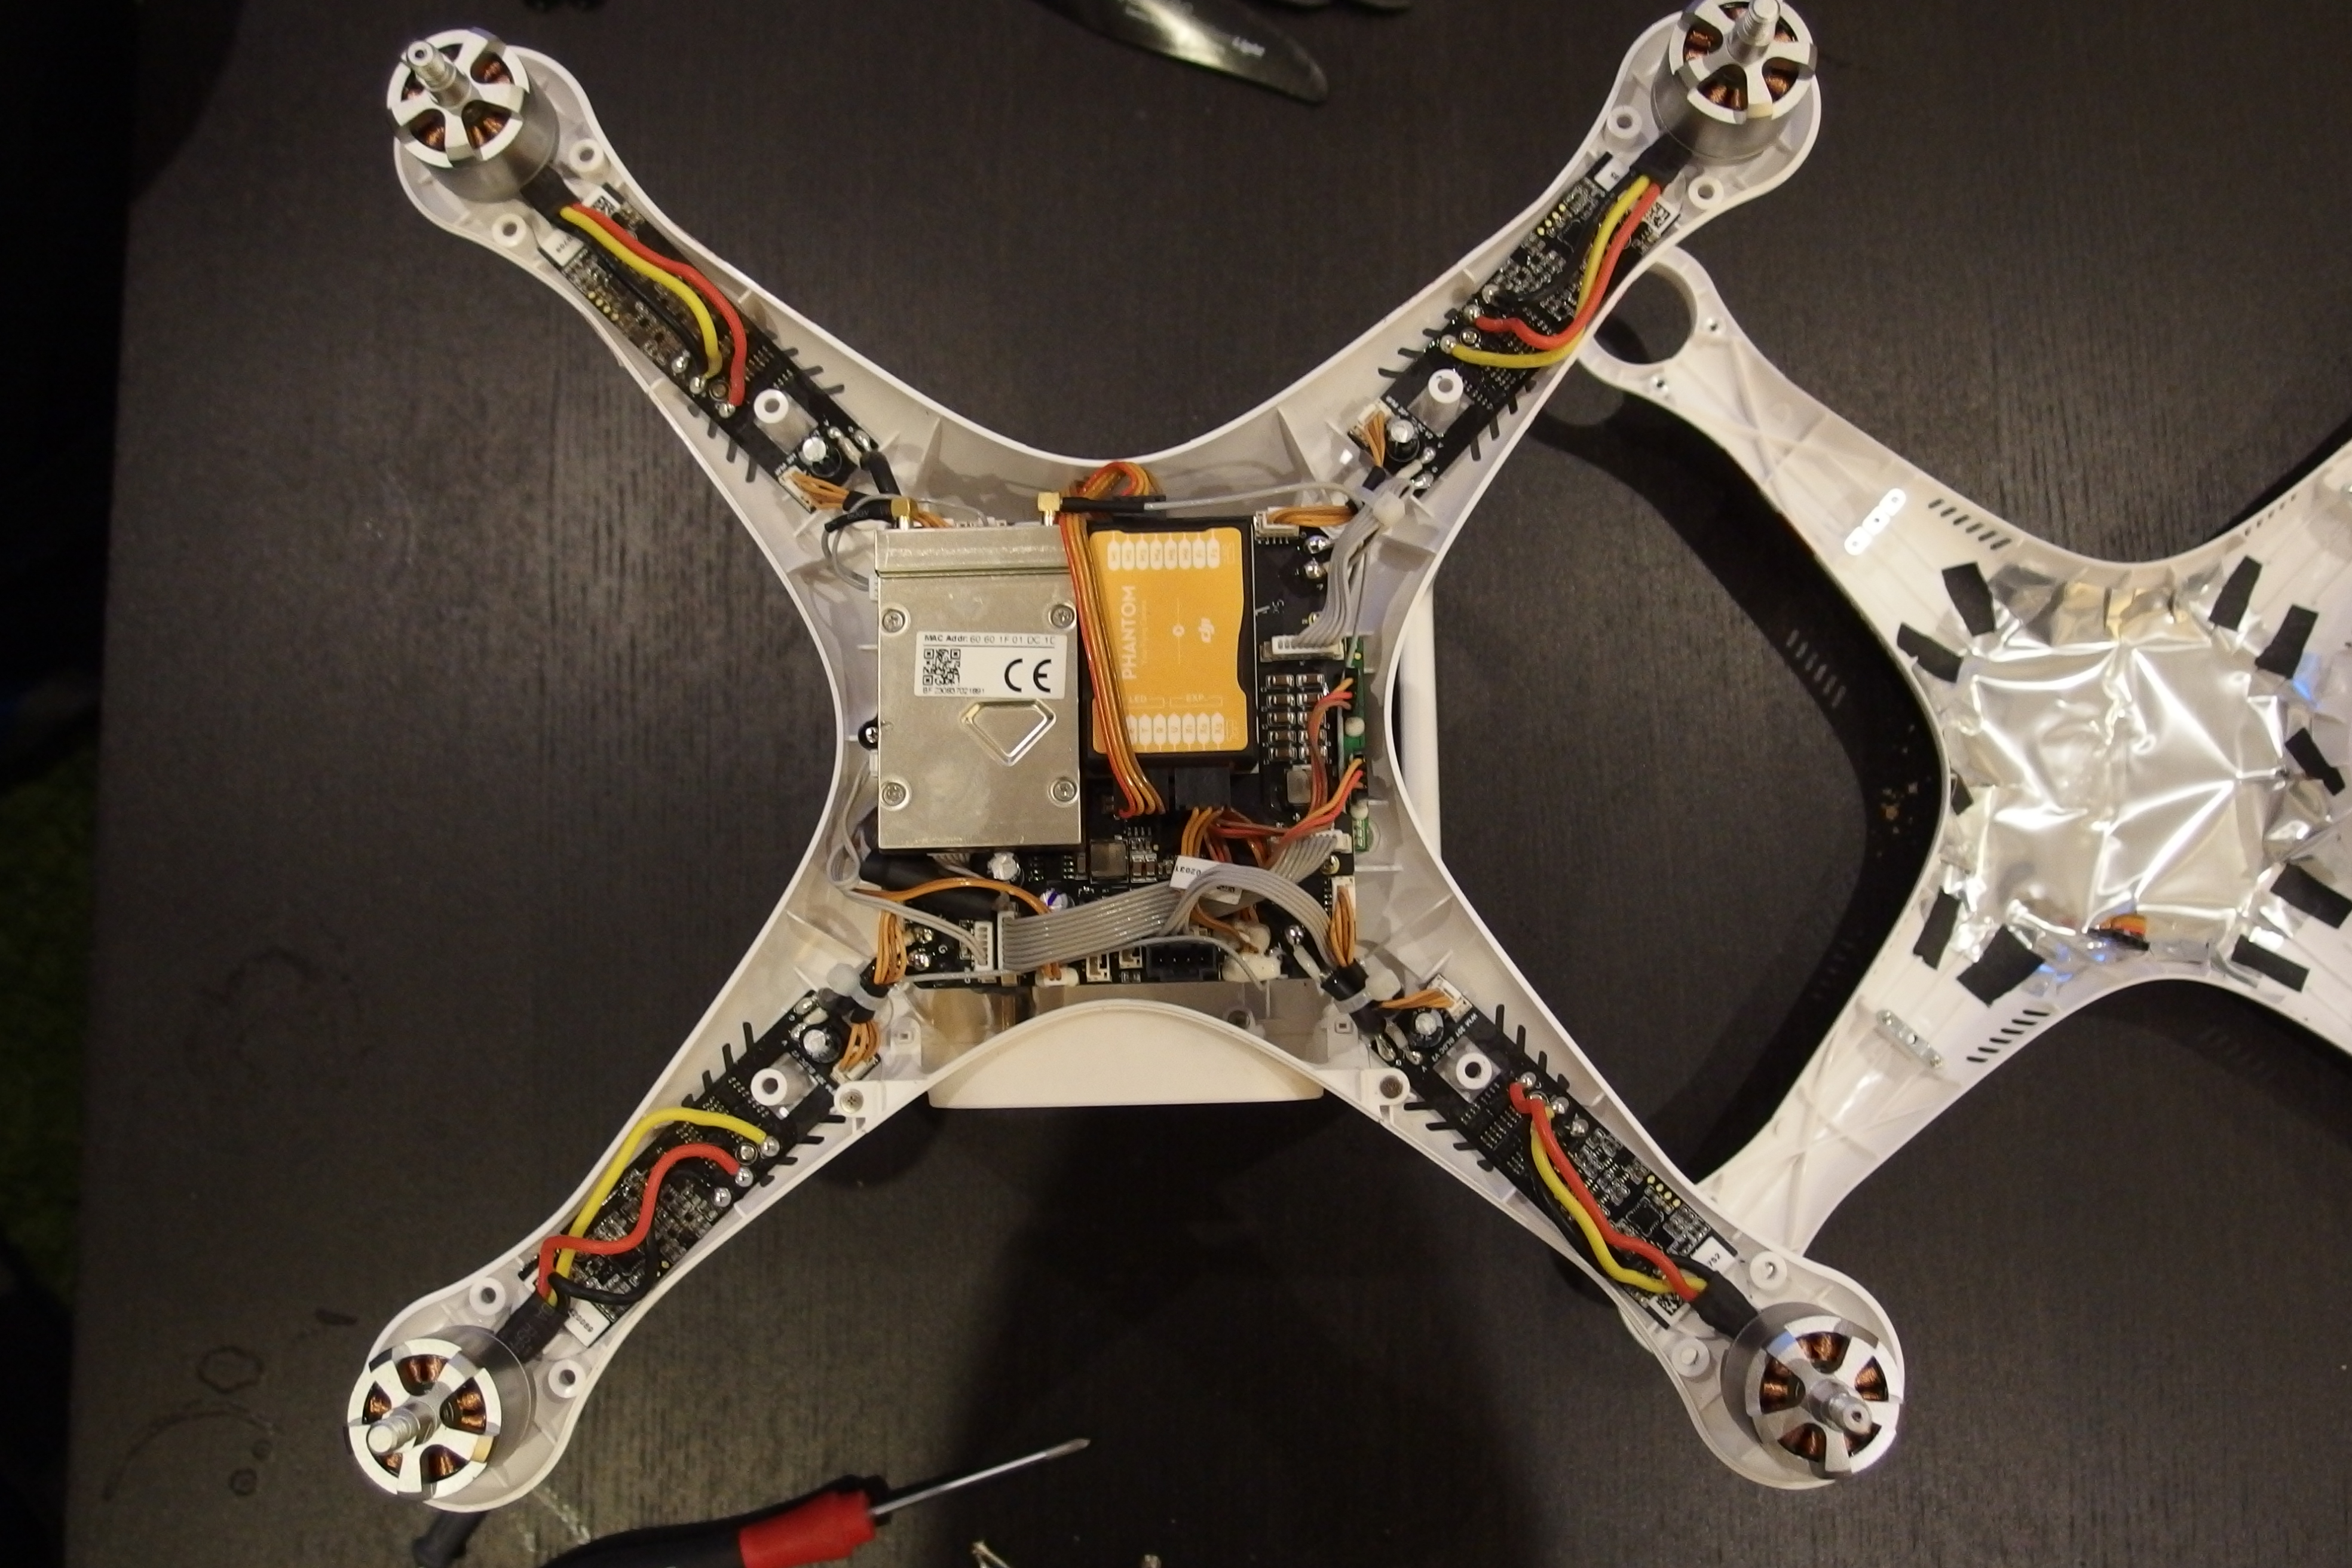
\includegraphics[width=0.55\textwidth]{img/dji/Dji1.jpg}
  \end{center}
  \label{dji}
  \caption{Eine offene DJI Phantom Vision 2 Plus.©eigenes}
\end{wrapfigure} In diesem Fall handelt es sich um einen Quadrocopter, der von vier Rotoren angetrieben wird. Die vier Rotoren sorgen für den stabilen Flug, sodass keine weiteren Steuertechniken nötig sind. Die Rotoren werden durch bürstenlose Motoren angetrieben (sogenannte \textit{Brushless-Motoren}), die direkt an den vier Armen befestigt sind. So muss die Kraft nicht über Wellen etc. an die Rotorblätter übergeben werden. 
\\
\\
\\
\\
\\
\\
\subsection{Sensoren und Steuergerät}

Damit ein Quadrocopter überhaupt fliegen kann, ist ein Zusammenspiel von diversen Sensoren und Steuergeräten nötig. Im folgenden Abschnitt werden die grundlegenden Bauteile näher beschrieben.\\
\subsubsection*{NAZA-M V2}
Das NAZA-M V2 ist das von DJI entwickelte Steuergerät des Kopters. In ihm laufen alle Sensorwerte und Steuersignale zusammen. Das NAZA-M steuert anhand dieser Messwerte die Drehzahl der vier Rotoren. Desweiteren hat es verschiedene Modi integriert die einen stabilen und sicheren Flug gewährleisten.\\
\subsubsection*{barometrischer Höhensensor}
Der Höhensensor misst anhand des Luftdrucks die derzeitige Höhe. Die Differenz zwischen Luftdruck bei Start und derzeitigem Luftdruck ergibt die Höhe. Diese Methode ist nicht sehr genau, da der Luftdruck Schwankungen unterliegt. In Zusammenspiel mit der Satellitennavigation funktioniert es aber zuverlässig.\\
\subsubsection*{\ac{GPS}}
Ein \ac{GPS} Empfänger erfasst den aktuellen Standort der Phantom 2 Plus. Über ihn ist ein autarker Flug anhand von vorher definierten Wegpunkten möglich. Die Phantom 2 Plus merkt sich den Startpunkt und kann bei ausfallen der Funkverbindung oder anderer Probleme selbständig zu diesem zurückkehren. Anhand des \ac{GPS} ist auch immer eine genaue Ausrichtung zu dem Piloten als Bezugspunkt möglich. Der \ac{GPS}-Empfänger ist direkt unter dem Deckel der Verkleidung angebracht um einen möglichst guten Empfang der \ac{GPS}-Signale zu gewährleisten.
\subsubsection*{Gyroskop}
Über ein Gyroskop, auch Kreiselinstrument genannt, kann die Ausrichtung des Flugobjektes erfasst werden. Der Vorwärtsflug des Phantom 2 Plus wird realisiert, indem die Drehzahl der Rotoren angepasst wird, sodass ein Kippen in Flugrichtung erfolgt. Anhand der Messdaten des Gyroskopes kann die Neigung gesteuert werden. Es wird um maximal 45° nach vorne gekippt, um ein \glqq Überkippen\grqq\ zu verhindern.\\
\subsubsection*{Accelerometer/Beschleunigungssensor}
Beschleunigungssensoren messen den Beschleunigungszuwachs bzw. die Abnahme der Beschleunigung. Zusammen mit dem Gyroskop sorgen sie für ein stabiles Flugbild. Die Bewegungsrichtung und Beschleunigung sind dem Steuergerät somit bekannt\cite{beschleunigung}.
\subsubsection*{Kompass}
Bei \ac{GPS} Navigation kann bei Stillstand/Schwebezustand die Ausrichtung des Objektes nicht genau bestimmt werden. Anhand eines Kompasses kann die Ausrichtung der Phantom 2 Plus auch im Schwebezustand einwandfrei für weitere Funktionen genutzt werden. Der Kompass ist extern an einem Bein des Kopters angebracht um mögliche Interferenzen mit den anderen elektronischen Bauteilen zu verhindern.\\
\subsubsection*{WLAN Sendeeinheit}
Über eine 2,4 GHz WLAN-Verbindung wird das Sucherbild der Kamera übertragen. Da die maximal in Deutschland zulässigen 100 mW nicht überschritten werden dürfen, ist ein Repeater an der Fernbedienung angebracht. Dieser empfängt das Signal und leitet es an ein Smartphone weiter. Das an der Fernbedienung montierte Smartphone liefert welches in der Lage ist das Bild der Kamera live zum fliegen bereitzustellen. Die Flug- und Gerätedaten wie Höhe, Akkuzustand und Speicherstand können über das Smartphone abgefragt werden. Die Ausrichtung der Kamera wird in horizontaler und vertikaler Neigung über den Touchscreen gesteuert. Die Reichweite wird mit ca. 500-700 Metern bei Sichtverbindung angegeben.
\subsubsection*{Funkverbindung}
Die Steuersignale der Funkfernbedienung werden über eine 6 Kanal 5.725-5.85 GHz Verbindung übertragen. Die Reichweite wird mit mindestens 700 Metern angegeben.
\subsubsection*{Kamera}
An einem 3D Gimbal, welcher anhand aller Lagesensoren die Verwacklungen durch den Flug ausgleicht, hängt eine Kamera mit 14 Megapixeln (Auflösung von 4384x3288 Pixel). Videoaufnahmen macht sie mit einer Auflösung von 1080p(1920x1080 Pixel). Das Bild des Suchers wird mit verminderter Auflösung direkt über die Wi-Fi-Verbindung auf das Smartphone des Piloten übertragen. Einstellungen wie Ausrichtung,Auflösung, Belichtung etc. lassen sich direkt über die Wi-Fi-Verbindung ansteuern.\\
\subsection{Flugfunktionen\cite{phantom}}
Es gibt eine Reihe von implementierten Funktionen die einen möglichst unkomplizierten Flug ermöglichen sollen. Im folgenden Abschnitt werden die Wichtigsten näher beschrieben.
\subsubsection*{Home-Lock Modus}
Das Quadcopter merkt sich anhand der GPS-Daten den Startpunkt/Home-Punkt, also den Standpunkt des Piloten. Wird im Flug der Home-Lock Modus gestartet, nimmt der Kopter den Home-Punkt als Bezugspunkt. Wird der Steuerknüppel nach rechts oder links gedrückt, zieht der Kopter einen Kreis mit dem Home-Punkt als Kreismittelpunkt. Wird der linke Steuerknüppel nach vorne bzw. hinten gedrückt, nähert/entfernt sich der Kopter dem Ausgangspunkt, egal in welche Richtung das Fluggerät gerade gedreht ist. Dies ist besonders praktisch wenn der Kopter sich nicht im nahen Sichtfeld befindet. Es ist auf weite Distanz schwer zu erkennen in welche Himmelsrichtung der Kopter ausgerichtet ist. Mithilfe vom Home-Lock Modus kann der Kopter aus jeder Lage wieder zum Piloten zurückgesteuert werden.
\subsubsection*{Course-Lock Modus}
Beim Course Lock wird die Ausrichtung beim Start gemerkt. Wird im Flug in den Course-Lock Modus schaltet, fliegt der Kopter immer mit Bezug auf diese Ausrichtung, unabhängig von der derzeitigen Ausrichtung.\\
\subsubsection*{Coming-Home/Failsafe Funktion}
Wenn der Kopter die Steuerfunkverbindung verliert z.B. durch leere Akkus in der Funkfernbedienung, ein Flug außerhalb des Empfangsbereiches, ein Flug hinter ein funkstörendes Objekt (Baum,Haus etc.) oder einen anderen Defekt, dann schaltet das Steuermodul in den Failsafe-Modus.
Ist die Verbindung verloren, wartet der Kopter schwebend an der derzeitigen Stelle auf neue Signale. Nach 10 Sekunden steigt er auf 20 Meter und steuert anhand der GPS Koordinaten zum Startpunkt zurück und landet.\\
